\begin{block}{Step 1: Finding Tensor Structure via Regression}
  \begin{itemize}
    \item {\bf Key Observation:} Regression on the powers of
        $(y,x)$ gives us the expected powers of the regression
        coefficients $\beta$. 
    \begin{columns}
      \begin{column}{0.65\textwidth}
  \begin{align*}
    y\tikzmark{regA} 
      &= \innerpp{\beta_h}{x} + \epsilon \\
      &= \mathmb{\ub{\innerp{\E[\beta_h]}{x}}_{\textrm{linear measurement}}} &&+ \mathmr{\ub{(\beta_h - \E[\beta_h])^T x + \epsilon}_{\textrm{noise}}} \\
    y^2 \tikzmark{regB}
      &= \left(\innerp{\beta_h}{x} + \epsilon\right)^2 && \\
      &= \mathmb{\innerpp{\ub{\E[\beta_h\tp{2}]}_{M_2}}{x\tp{2}}}
      &&+ \mathmg{\textrm{bias}_2} + \mathmr{\textrm{noise}_2} \\
    y^3 \tikzmark{regC}
    &= \mathmb{\innerpp{\ub{\E[\beta_h\tp{3}]}_{M_3}}{x\tp{3}}} &&+ \mathmg{\textrm{bias}_3} + \mathmr{\textrm{noise}_3}
  \end{align*}
    \end{column}
      \begin{column}{0.25\textwidth}
  \begin{tikzpicture}
    \point{mark}{(0,0)};
      \regressionA{($(mark) + (0,0cm)$)};
      \regressionB{($(mark) + (0,-2.5cm)$)};
      \regressionC{($(mark) + (0,-4.5cm)$)};
  \end{tikzpicture}
    \end{column}
  \end{columns}


\item $M_2$ and $M_3$ are both of rank $k$, so we can use low rank regression$^{3,4}$!
  \begin{align*}
    \hat M_2 
      &= \arg\min_{M} \sum_{(x,y)\in\mathcal{D}} 
        \left( y^2 - \innerp{M}{x\tp{2}} - \textrm{bias}_2\right)^2 
          + \lambda_2 \mathmb{\ub{\|M\|_{*}}_{\sum_i \sigma_i(M)}}\\
    \hat M_3 
      &= \arg\min_{M} \sum_{(x,y)\in\mathcal{D}} 
        \left( y^3 - \innerp{M}{x\tp{3}} - \textrm{bias}_3\right)^2 
        + \lambda_3 \|M\|_{*}
  \end{align*}
  \end{itemize}

  \footnotesize{%
  \hfill
    [3] Fazel, 2002; [4] Tomoika, Hayashi and Kashima, 2010
  }

\end{block}

\begin{block}{Step 2: Parameter Recovery via Tensor Factorization}
  \begin{itemize}
      \item $M_3$ has a low-rank tensor decomposition:
      $M_3 = \sum_{h=1}^k \pi_h \beta_h\tp{3}$
      \vspace{1ex}\\
      \begin{tikzpicture}[scale=1.5]
          \tensorfactorization{(0cm,0cm)};
      \end{tikzpicture}

    \item {\bf Key Observation:} If $\beta_h$ are orthogonal, they are eigenvectors$^{5}$; 
      $M_3(\beta_h,\beta_h) = \pi_{h} \beta_{h}$.
    \item In general, we can whiten $M_3$ first.
  \end{itemize}
  \footnotesize{%
  \hfill
  [5]: Anandkumar, Ge, Hsu, Kakade, Telgarksy, 2012.
  }

\end{block}

\begin{block}{Experiments}
  \begin{itemize}
      \item With finite samples, Spectral Experts seems to find parameters
        that sufficiently separate components that EM initialized with
        these parameters recovers true parameters more often than EM with random initializations.
  \item In this example, $y = \beta^T [ 1, t, t^4 ,t^7 ]^T + \epsilon$. $k = 3, d = 4, n = 10^5$,
  \begin{tikzpicture}
    \node (graphs) {%
      \includegraphics[width=0.3\textwidth,height=5cm,keepaspectratio]{figures/EM-1833.pdf}
      \includegraphics[width=0.3\textwidth,height=5cm,keepaspectratio]{figures/Spectral-Spectral+EM-1833.pdf}
      \includegraphics[width=0.3\textwidth,height=5cm,keepaspectratio]{figures/EM-Spectral-Spectral+EM-hist.pdf}
      };
  \end{tikzpicture}
  \item Below are parameter errors averaged over 10 initializations on
    10 different simulated datasets with the specified parameter
    configurations,
    \begin{tikzpicture}
      \node (exp1) {\includegraphics[width=0.2\textwidth]{figures/err-hist-0.pdf}};
      \node[scale=0.8,below=-0.2cm of exp1] {$d=4, k=2$};
      \node[right=0cm of exp1] (exp2) {\includegraphics[width=0.2\textwidth]{figures/err-hist-1.pdf}};
      \node[scale=0.8,below=-0.2cm of exp2] {$d=5, k=2$};
      \node[right=0cm of exp2] (exp3) {\includegraphics[width=0.2\textwidth]{figures/err-hist-2.pdf}};
      \node[scale=0.8,below=-0.2cm of exp3] {$d=5, k=3$};
      \node[right=0cm of exp3] (exp4) {\includegraphics[width=0.2\textwidth]{figures/err-hist-3.pdf}};
      \node[scale=0.8,below=-0.2cm of exp4] {$d=6, k=2$};
    \end{tikzpicture}

  \item {\bf Log-likelihood cartoon:} It seems that our parameter estimates fall in the right basin of attraction for EM.\\
      \begin{tikzpicture}
        \point{mark}{(0,0)}
        % x, y
        \llhood{4cm}{0};

        \node[scale=0.3,circle,fill=red] at (em2) {};
        \node at ($(em2) + (0.7cm,0)$) {$\mathmr{\hat\theta_{\textrm{EM}}}$};
        \draw[-latex,smooth,line width=1pt,red] ($(em2-start) + (+0.1cm,+0.05cm)$) -- ($(em2) + (+0.15cm,0.00cm)$);
        %\draw[dashed,red,line width=0.7pt] ($(em2)-(3.5cm,0)$) -- ($(em2)+(0.5cm,0)$);

    %    \draw<3>[latex-latex,DarkGreen,line width=1pt,dashed] ($(mle) + (-1.2cm,0.8cm)$) -- node[above]{$\mathmg{\epsilon}$} ($(mle) + (+1.2cm,0.8cm)$);
        \node[scale=0.3,circle,fill=DarkGreen] at (spec) {};
        \node at ($(spec) + (0.6cm,0.3cm)$) {$\mathmg{\hat\theta_{\textrm{spec}}}$};
        %\draw[dashed,DarkGreen,line width=0.7pt] ($(spec)-(0.5cm,0)$) -- ($(spec)+(3.5cm,0)$);

        \draw[-latex,smooth,line width=1pt,DarkGreen] ($(spec) + (-0.1cm,+0.05cm)$) -- ($(mle) + (-0.30cm,+0.10cm)$);
        \node[scale=0.3,circle,fill=blue] at (mle) {};
        \node[anchor=west] at ($(mle) + (0.2cm,0)$) {$\mathmb{\hat\theta}_{\textrm{spec + EM}}$};

        %\draw[dashed,blue,line width=0.7pt] ($(mle)-(0.4cm,0)$) -- ($(mle)+(0.4cm,0)$);
      \end{tikzpicture}
  \end{itemize}
  \vspace{-1ex}

\end{block}

\begin{block}{Future Work}
  \begin{itemize}
    \item How can we handle other discriminative models?
      \begin{itemize}
          \item Non-linear link functions (hidden variable logistic regression).
          \item Dependencies between $h$ and $x$ (mixture of experts).
      \end{itemize}
  \end{itemize}

\end{block}


\vfill

